\documentclass{beamer}
\usetheme{Warsaw}
\usepackage{nhtvslides}
\usepackage{graphicx}
\usepackage{listings}
\lstset{language=CAML,
basicstyle=\ttfamily\footnotesize,
frame=shadowbox,
breaklines=true}
\usepackage[utf8]{inputenc}
\DeclareMathOperator{\lerp}{lerp}

\title{Building a physics engine - part 2: narrow phase of collision detection}

\author{Dr. Giuseppe Maggiore}

\institute{NHTV University of Applied Sciences \\ 
Breda, Netherlands}

\date{}

\begin{document}
\maketitle

\begin{frame}{Table of contents}
\tableofcontents
\end{frame}

\section{Narrow phase collision detection and response}
\begin{slide}{Narrow phase}{Narrow phase}{
\item Find intersections for each pair of rigid bodies
\begin{itemize}
\item Whether they intersect
\item When they intersect
\item Where they intersect
\end{itemize}
\item Acceptable precision
\item Very high performance
}\end{slide}

\begin{slide}{Narrow phase}{Response}{
\item At all points of contact the \textit{relative velocity} projected along the normal must be non-negative
\item No pair of bodies in contact is getting closer
\begin{itemize}
\item This would mean that they are penetrating each other
\end{itemize}
}\end{slide}

\begin{frame}{Relative Velocity}
\center
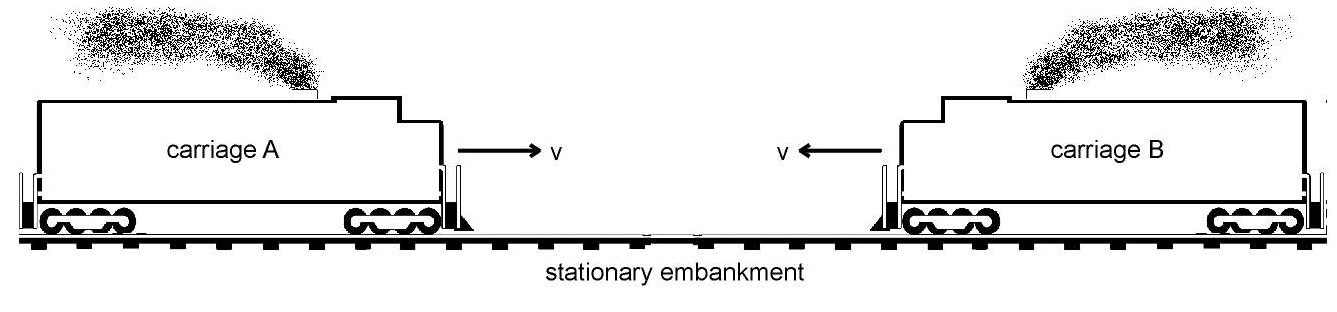
\includegraphics[width=8cm]{Pics/Rel_Vel.png}
\end{frame}

\begin{slide}{Narrow phase}{Response}{
\item \textit{Relatively} easy to handle between pairs of bodies
\item Multiple bodies in contact make it much harder
}\end{slide}

\begin{frame}{Relative Velocity}
\center
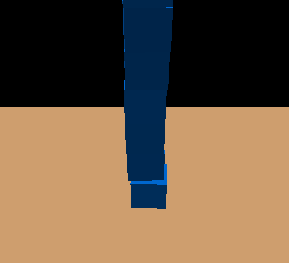
\includegraphics[width=6cm]{Pics/Stacking.png}
\end{frame}

\section{Convex polyhedra}
\begin{slide}{Convex polyhedra}{Convex polyhedra}{
\item Also known as \textit{polytopes}
\item $\forall P,Q \in C. \forall \alpha \in [0..1]. \lerp(\alpha, P, Q) \in C$
\item Complex bodies can be treated as multiple polytopes with distance constraints
}\end{slide}

\begin{frame}{Convex polygon}
\center
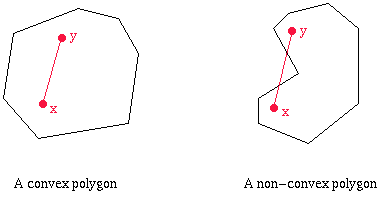
\includegraphics[width=6cm]{Pics/ConvexPolyhedron.png}
\end{frame}

\begin{frame}{Convex polyhedra}
\center
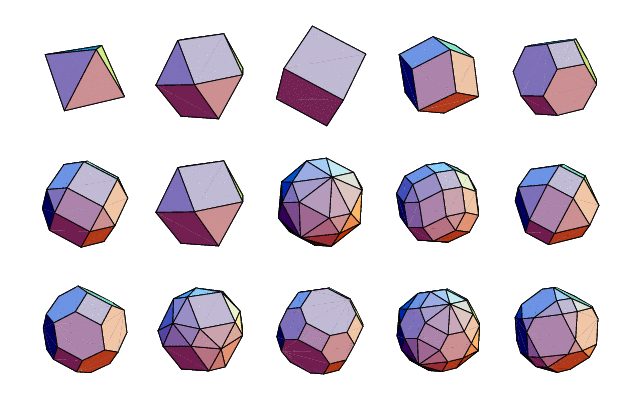
\includegraphics[height=5cm]{Pics/ConvexPolyhedra.png}
\end{frame}

\section{Separating axis}
\begin{slide}{Separating axis}{Method of separating axis}{
\item We use a method that works in 2D and 3D
\begin{itemize}
\item We look for an axis/plane that separates the bodies
\end{itemize}
}\end{slide}

\begin{frame}{Separating axis}
\center
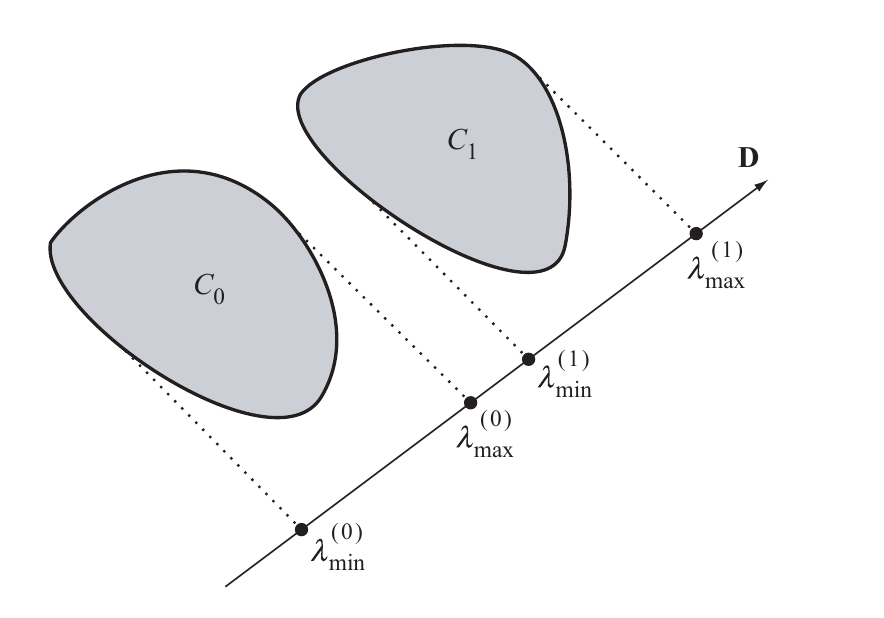
\includegraphics[height=5cm]{Pics/Fig6_19.png}
\end{frame}

\begin{slide}{Separating axis}{Method of separating axis}{
\item Given a (not necessarily unit-length) direction $D$ and two polytopes $C_0$ and $C_1$
\item We project them over the direction $D$: $I_i = [\lambda_{min}^i,\lambda_{max}^i] = [\min_{x\in C_i}\{ D \cdot (X-O) \}, \max_{x\in C_i}\{ D \cdot (X-O) \}]$
\item There is no collision if $\exists D . \lambda_{min}^0 > \lambda_{max}^1 \vee \lambda_{min}^1 > \lambda_{max}^0$
}\end{slide}

\begin{frame}{Separating axis}
\center
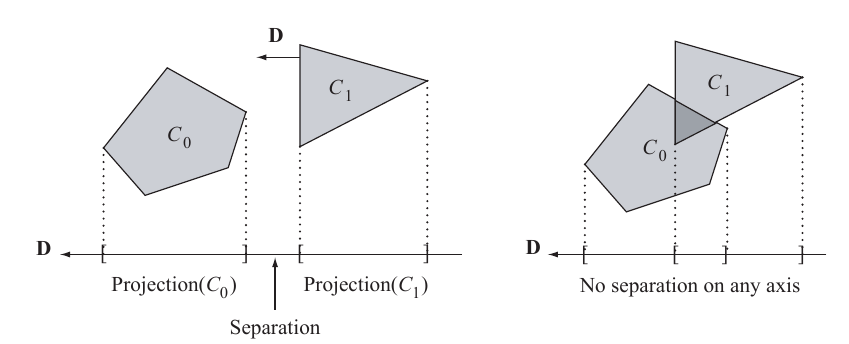
\includegraphics[width=8cm]{Pics/Fig6_20.png}
\end{frame}

\begin{slide}{Separating axis}{Method of separating axis}{
\item $D$ may be multiplied by a (non-zero) constant
\item The projection is scaled uniformly, but no contact still translates into a separated projection
\item The translation of a separating axis remains a separating axis, so we only deal with lines that go through the origin
}\end{slide}

\begin{frame}{Scale of separating axis}
\center
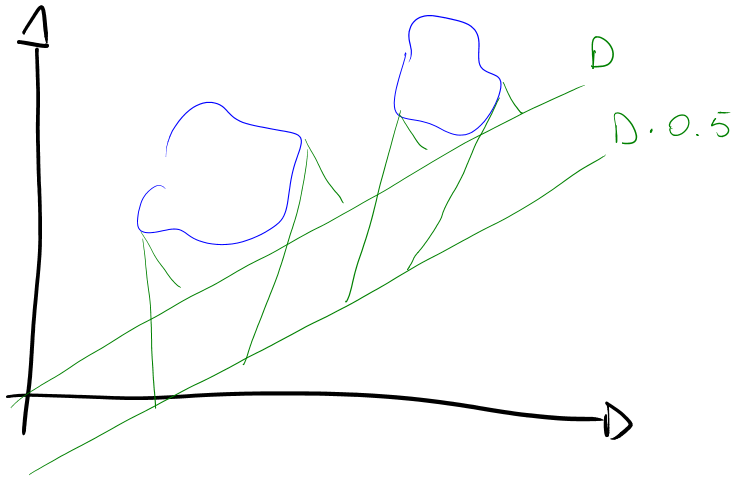
\includegraphics[width=8cm]{Pics/ScaleOfSeparatingAxis.png}
\end{frame}

\begin{frame}{Translation of separating axis}
\center
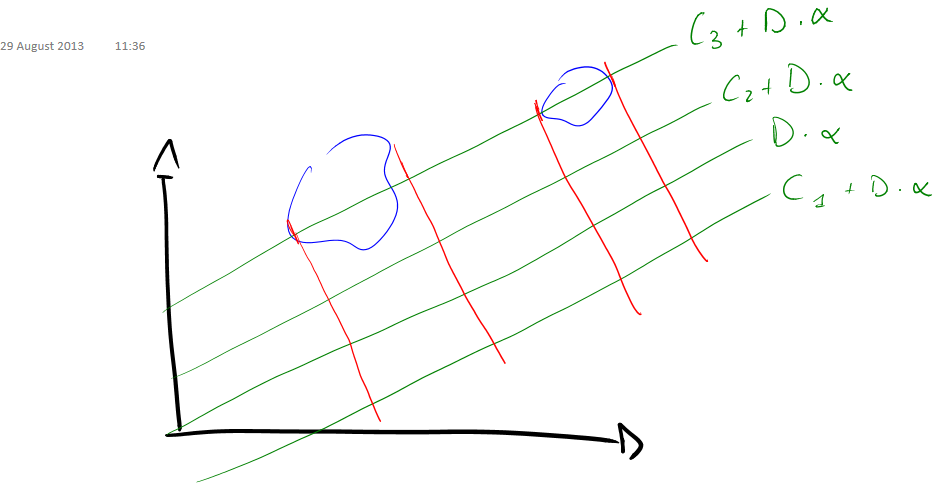
\includegraphics[width=8cm]{Pics/TranslationOfSeparatingAxis.png}
\end{frame}

% FIG OF SCALED/TRANSLATED PROJECTION

\begin{slide}{Separating axis}{Method of separating axis}{
\item We now consider $C_j$ polytopes, each with
\begin{itemize}
\item $P_i^j$ vertices, \textit{ordered counter-clockwise} and with wrapping indices
\item $E_i^j = P_{i+1}^j - P_i^j$ edges, \textit{ordered counter-clockwise}
\item $N_i^j$ normals, perpendicular to the edges
\end{itemize}
\item Similarly we store the triangles in 3D
}\end{slide}

\begin{slide}{Separating axis}{Method of separating axis}{
\item There are infinite candidate directions $D$
\item Fortunately we need only consider a finite set
\item In 2D, the normals of each polygon
}\end{slide}

\begin{frame}{Separating axis}
\center
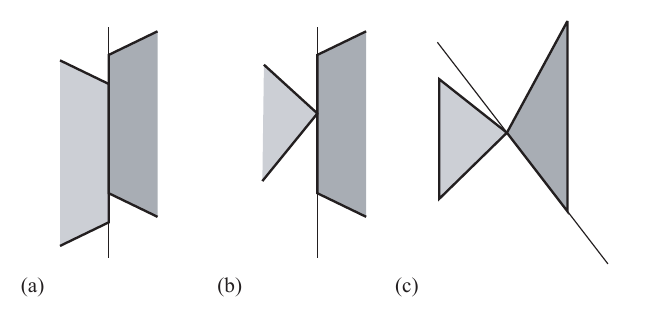
\includegraphics[width=8cm]{Pics/SeparatingAxesIn2D.png}
\end{frame}

\begin{slide}{Separating axis algorithms}{Algorithms}{
\item Naïve algorithm
\item For each normal:
\begin{itemize}
\item Project all vertices of both polytopes
\item Compute the intervals
\item Check for intersection
\end{itemize}
}\end{slide}

\begin{slide}{Separating axis algorithms}{Algorithms}{
\item Smarter algorithm
\begin{itemize}
\item For each body $C_j$
\item For each normal $P_i^j, N_i^j$
\item Check if the closest vertex $P_k^l$ of the other body $C_l$ is too close to the edge
\item $(P_k^l - P_i^j) \cdot N_i^j > \epsilon$
\end{itemize}
}\end{slide}

\begin{frame}{Separation against face}
\center
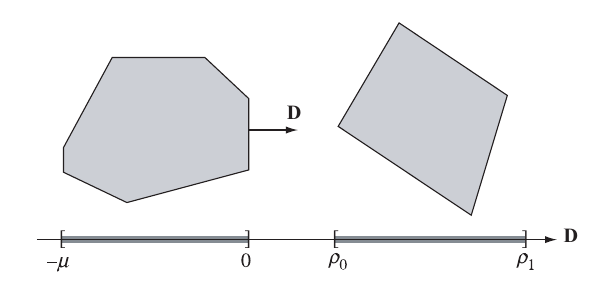
\includegraphics[height=5cm]{Pics/SeparationOfVertex.png}
\end{frame}

\begin{frame}[fragile]{Pseudo-code}
\begin{lstlisting}
bool TestIntersection (ConvexPolygon C0, ConvexPolygon C1) { 
  for (i0 = C0.GetN()-1, i1 = 0; i1 < C0.GetN(); i0 = i1++) { 
    P = C0.GetVertex(i1);
    D = C0.GetNormal(i0); 
    if (WhichSide(C1,P,D) > 0) { 
      return false; 
    }
  }
\end{lstlisting}
\end{frame}
\begin{frame}[fragile]{Pseudo-code}
\begin{lstlisting}
  for (i0 = C1.GetN()-1, i1 = 0; i1 < C1.GetN(); i0 = i1++) { 
    P = C1.GetVertex(i1); 
    D = C1.GetNormal(i0); 
    if (WhichSide(C0,P,D) > 0) { 
      return false; 
    } 
  }
  return true;
}
\end{lstlisting}
\end{frame}
\begin{frame}[fragile]{Pseudo-code}
\begin{lstlisting}
int WhichSide (ConvexPolygon C, Point P, Vector D) { 
  posCount = 0; 
  negCount = 0; 
  zeroCount = 0; 
  for (i = 0; i < C.GetN(); ++i) { 
    t = Dot(D,C.GetVertex(i) - P); 
    if (t > 0) { posCount++; } 
    else if (t < 0) { negCount++; } 
    else { zeroCount++; }    
    if ((posCount > 0 and negCount > 0) or zeroCount > 0) { return 0; }
  } 
  return posCount ? 1 : -1;
}  
\end{lstlisting}
\end{frame}

\begin{slide}{Separating axis algorithms}{Optimizations}{
\item Bisection on the sorted vertices
\item Find the vertex closest to an edge faster
}\end{slide}

\begin{slide}{Separating axis algorithms}{Optimizations}{
\item 2D and 3D: BSP, Gauss map, hash table of the vertices sorted w.r.t. their direction
\item Find the vertex closest to an edge much faster
\item We will \textit{maybe} see this algorithm, depending on how fast the course goes
}\end{slide}

\begin{slide}{Separating axis in 3D}{Candidate axes}{
\item In 2D the candidate axes are just the edge normals
\item In 3D the face normals are not enough
\item Edge-to-edge collisions are not covered
}\end{slide}

\begin{frame}{Separating axis}
\center
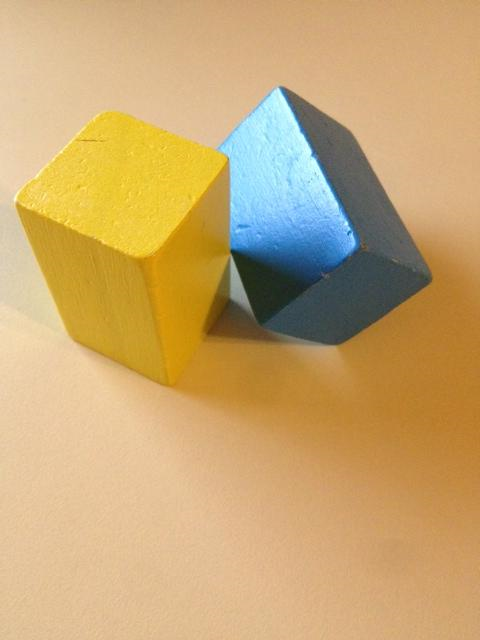
\includegraphics[height=5cm]{Pics/EdgeToEdgeCross.png}
\end{frame}

\begin{slide}{Separating axis in 3D}{Candidate axes}{
\item Also consider edge-to-edge cross products
\item Exactly the same algorithm, but with more potential axes
}\end{slide}

\begin{frame}{Separating axis}
\center
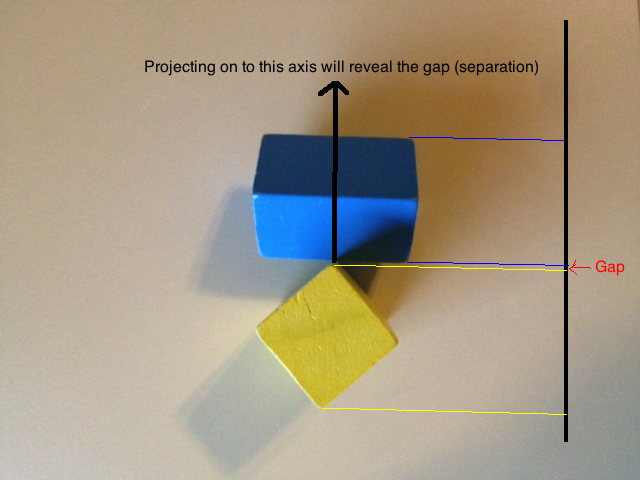
\includegraphics[height=5cm]{Pics/EdgeToEdgeCross2.png}
\end{frame}

\begin{frame}[fragile]{Pseudo-code}
\begin{lstlisting}
bool TestIntersection (ConvexPolyhedron C0, ConvexPolyhedron C1) { 
  for (i = 0; i < C0.GetFCount(); ++i) { 
    D = C0.GetNormal(i); 
    ComputeInterval(C0,D,min0,max0);    
    ComputeInterval(C1,D,min1,max1); 
    if (max1 < min0 || max0 < min1) { return false; }
  }
\end{lstlisting}
\end{frame}
\begin{frame}[fragile]{Pseudo-code}
\begin{lstlisting}  
  for (j = 0; j < C1.GetFCount(); ++j) { 
    D = C1.GetNormal(j); 
    ComputeInterval(C0,D,min0,max0); 
    ComputeInterval(C1,D,min1,max1); 
    if (max1 < min0 || max0 < min1) { return false; } 
  }
\end{lstlisting}
\end{frame}
\begin{frame}[fragile]{Pseudo-code}
\begin{lstlisting}
  for (i = 0; i < C0.GetECount(); ++i) { 
    for (j = 0; j < C1.GetECount(); ++j) { 
      D = Cross(C0.GetEdge(i),C1.Edge(j)); 
      ComputeInterval(C0,D,min0,max0); 
      ComputeInterval(C1,D,min1,max1); 
      if (max1 < min0 || max0 < min1){ return false; }
    } 
  }
  return true;
}
\end{lstlisting}
\end{frame}
\begin{frame}[fragile]{Pseudo-code}
\begin{lstlisting}
void ComputeInterval (ConvexPolyhedron C, Vector D, double& min, double& max) { 
  min = Dot(D,C.GetVertex(0)); 
  max = min; 
  for (i = 1; i < C.GetVCount(); ++i) { 
    value = Dot(D,C.GetVertex(i)); 
    if (value < min) {
      min = value;
    } else { 
      max = value; 
    }
  }
}
\end{lstlisting}
\end{frame}

\section{Moving objects}
\begin{slide}{Moving objects}{Moving objects}{
\item Objects are usually moving in a game :)
\item We must check for future intersections
\item With some simplifying assumptions 
\begin{itemize}
\item Rotations can be ignored (phew!)
\item Interpenetration may happen a bit
\end{itemize}
}\end{slide}

\begin{slide}{Moving objects}{Moving objects}{
\item Use the \textit{moving projection} on an axis
\item Consider the \textit{relative velocity} $V = V_2 - V_1$
\item Speed of projection along $D$ is $\sigma = V \cdot D$ when $|D| = 1$
\item The distance of the minimum point must be bigger than $\sigma$
\item $\Delta x = \sigma \Delta t$ $\Delta t \frac{\Delta x}{d} = $ time of collision
\item When the time of collision is outside the time of the current frame, then there is no collision
}\end{slide}

\begin{frame}[fragile]{Moving objects}
\begin{lstlisting}
bool TestIntersection (ConvexPolygon C0, Vector V0, ConvexPolygon C1, Vector V1, double tmax, double& tfirst, double& tlast) { 
  V = V1 - V0;
  tfirst = 0; 
  tlast = INFINITY;
\end{lstlisting}
\end{frame}
\begin{frame}[fragile]{Pseudo-code}
\begin{lstlisting}
  for (i0 = C0.GetN() - 1, i1 = 0; i1 < C0.GetN(); i0 = i1++) { 
    D = C0.GetNormal(i0); 
    ComputeInterval(C0,D,min0,max0);
    ComputeInterval(C1,D,min1,max1); 
    speed = Dot(D,V); 
    if (NoIntersect(tmax,speed,min0,max0,min1,max1,tfirst, tlast)) { return false; }
  }
\end{lstlisting}
\end{frame}
\begin{frame}[fragile]{Pseudo-code}
\begin{lstlisting}  
  for (i0 = C1.N - 1, i1 = 0; i1 < C1.N; i0 = i1++) { 
    D = C1.GetNormal(i0); 
    ComputeInterval(C0,D,min0,max0); 
    ComputeInterval(C1,D,min1,max1); 
    speed = Dot(D,V); 
    if (NoIntersect(tmax,speed,min0,max0,min1,max1,tfirst, tlast)) { return false; } 
  } 
  return true;
}
\end{lstlisting}
\end{frame}

\begin{slide}{Moving objects}{Moving objects}{
\item if the polygons intersect at a first time $t_{\text{first}}$, then there is a separating axis $\forall t. t < t_{\text{first}}$
\item if the polygons intersect at a last time $t_{\text{last}}$, then there is a separating axis $\forall t. t > t_{\text{last}}$
\item if for all direction $t_{\text{first}} < t_{\text{last}}$, then the polygons intersect at time $t_{\text{first}}$ (check against $\Delta t$)
\item if for all direction $t_{\text{first}} > t_{\text{last}}$, then the polygons do not intersect (all axis must intersect at the same time!)
}\end{slide}

\begin{frame}[fragile]{Pseudo-code}
\begin{lstlisting}
bool NoIntersect (double tmax, double speed, double min0, double max0, double min1, double max1, double& tfirst, double& tlast) { 
  if (max1 < min0) {
    if (speed <= 0) { return true; }
    t = (min0 - max1)/speed; 
    if (t > tfirst) { tfirst = t; } 
    if (tfirst > tmax) { return true; }
    t = (max0 - min1)/speed; 
    if (t < tlast) { tlast = t; } 
    if (tfirst > tlast) { return true; }
\end{lstlisting}
\end{frame}
\begin{frame}[fragile]{Pseudo-code}
\begin{lstlisting}
  } else if ( max0 < min1 ) { 
    if (speed >= 0) { return true; }
    t = (max0 - min1)/speed; 
    if (t > tfirst) { tfirst = t; } 
    if (tfirst > tmax) { return true; }
    t = (min0 - max1)/speed; 
    if (t < tlast) { tlast = t; } 
    if (tfirst > tlast) { return true; }
\end{lstlisting}
\end{frame}
\begin{frame}[fragile]{Pseudo-code}
\begin{lstlisting}
  } else {
    if (speed > 0) { 
      t = (max0 - min1)/speed;
      if (t < tlast) { tlast = t; } 
      if (tfirst > tlast) { return true; }
    } else if (speed < 0) { 
      t = (min0 - max1)/speed; 
      if (t < tlast) { tlast = t; } 
      if (tfirst > tlast) { return true; } 
    }
  } 
  return false;
}
\end{lstlisting}
\end{frame}

\section{Finding the contact manifold}
\begin{slide}{Finding intersections}{Contact manifold}{
\item The collision response system needs the intersections
\item So far we have built \texttt{TestIntersection}
\item Huge numbers of possible algorithms for this (\textbf{GJK} is the most diffuse)
\item We now \textit{sketch} a description of one intuitive algorithm
}\end{slide}

\begin{slide}{Finding intersections}{Finding intersections}{
\item When the intersection is found at time $T$, before returning
\item We move the bodies forward with the respective velocities
\item We compute and return (an approximation) of the contact set
\item May be face-to-vertex or edge-to-edge
}\end{slide}

\begin{slide}{Finding intersections}{Finding intersections for SAT failures}{
\item Identify \textit{reference face} ($D=N$) and \textit{incident face} (most anti-parallel to $D$)
\item Clip incident face against edges of reference face
\item Keep all resulting vertices \textit{below or on} the reference face
}\end{slide}

\begin{frame}{Reference face}
\center
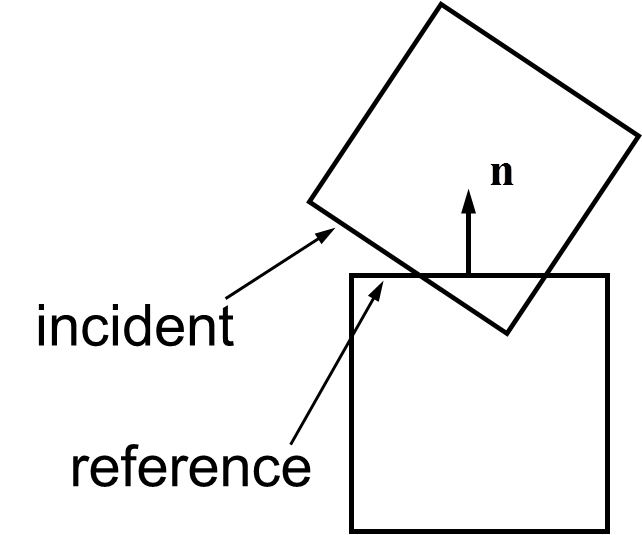
\includegraphics[height=5cm]{Pics/ReferenceFace.png}
\end{frame}

\begin{frame}{Reference face sideways}
\center
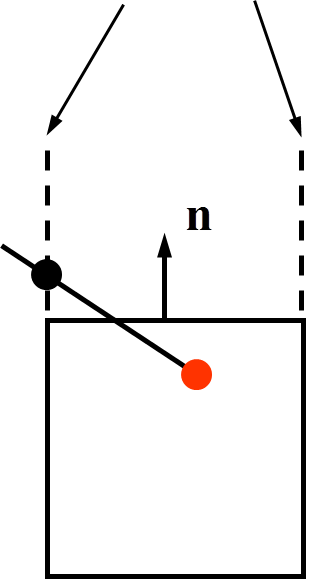
\includegraphics[height=5cm]{Pics/ReferenceFaceSideways.png}
\end{frame}

\begin{slide}{Finding intersections}{Edge-to-edge SAT failures}{
\item Just intersect the edges
}\end{slide}

\begin{slide}{Finding intersections}{Contact manifold}{
\item Two vertices are enough in 2D
\item Three vertices are enough in 3D
\item Too many more vertices do not improve stability (a few might)
\item We always choose the ones penetrating the most
\item Deterministic as much as possible (contact caching)
}\end{slide}

\begin{frame}{Contact manifold}
\center
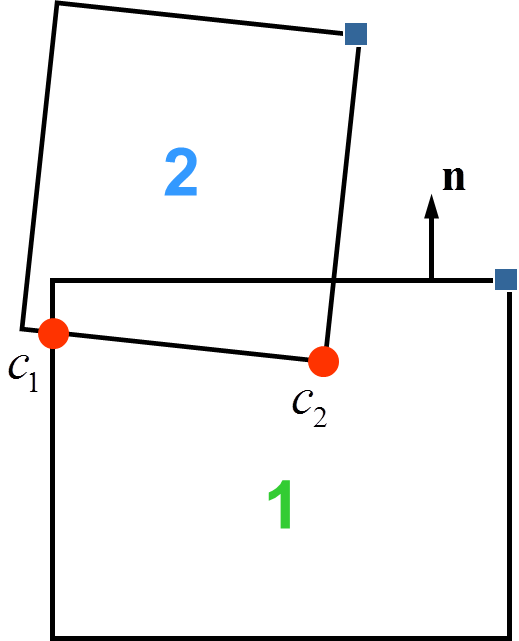
\includegraphics[height=5cm]{Pics/ContactManifold.png}
\end{frame}

\begin{slide}{Finding intersections}{Clipping and intersections}{
\item Sutherland-Hogman algorithm for clipping
\item Edge-to-edge intersection
}\end{slide}

\begin{slide}{Finding intersections}{Clipping faces}{
\item Project planes from the edges of the reference face
\item Vertices of the incident face \textit{inside} all planes are contact points
\item Reference plane with incident edge intersections are more contact points
\item Keep a subset of the points: (most inside the reference face)
}\end{slide}

\begin{slide}{Finding intersections}{Clipping a vertex}{
\item Given a plane $\langle N,d \rangle$ where $N$ is the normal of the plane and $d$ is the minimum distance of the plane from the origin
\item We determine the side of the plane on which a vertex $V$ lies with the sign of $P \cdot N - d$
}\end{slide}

\begin{frame}{Clipping}
\center
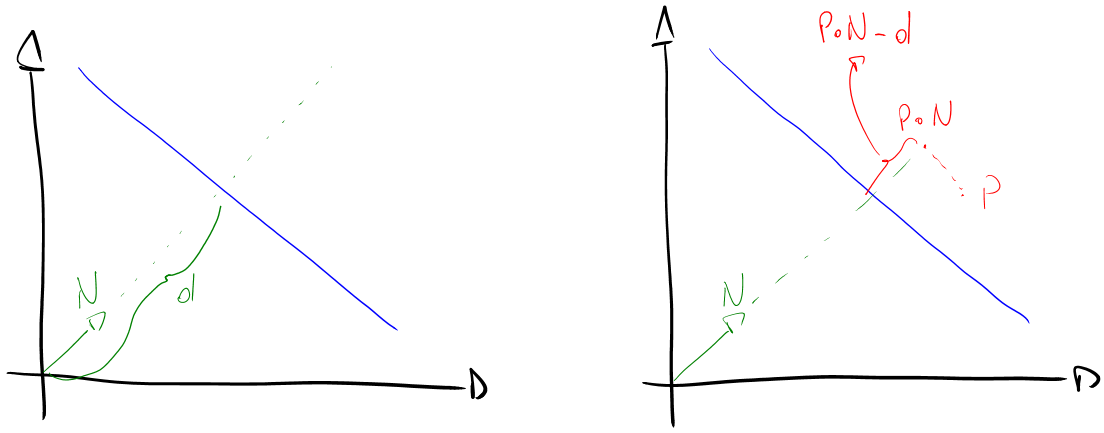
\includegraphics[width=10cm]{Pics/PlaneVertexClipping.png}
\end{frame}

\begin{slide}{Finding intersections}{Clipping a vertex}{
\item All signs of plane-vertex distance must be the same
\item The planes must all be facing inward (or outward)
}\end{slide}

\begin{slide}{Finding intersections}{Clipping an edge}{
\item Given a plane $\langle V \cdot N = d \rangle$ and an edge $V = A + \alpha B$ ($0 \leq \alpha \leq 1$)
\item We put these equations together: $(A + \alpha B) \cdot N = d$ and solve for $\alpha = \frac{d - A \cdot N}{B \cdot N}$
}\end{slide}

\begin{slide}{Finding intersections}{Clipping an edge}{
\item $\alpha = \frac{d - A \cdot N}{B \cdot N}$
\item Watch for lack of solutions
\begin{itemize}
\item If $|B \cdot N| \leq \epsilon$ then edge and plane are parallel
\item No intersection possible
\end{itemize}
}\end{slide}

\begin{frame}{Clipping}
\center
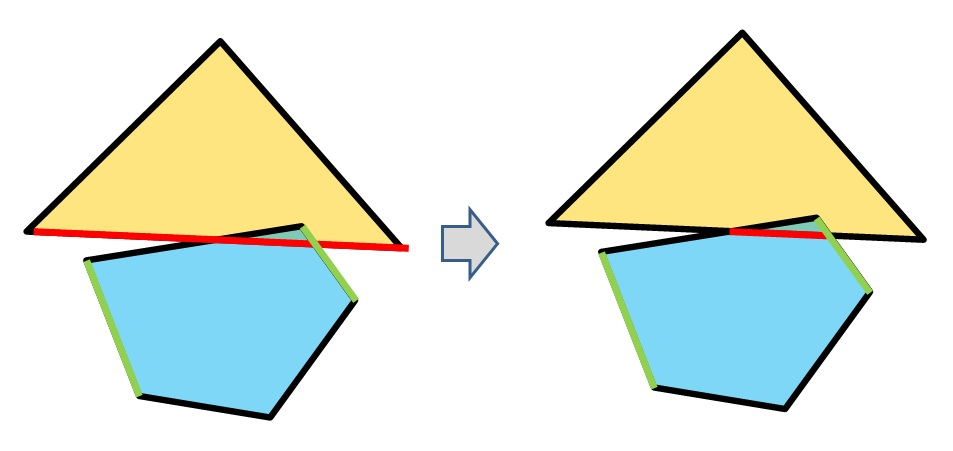
\includegraphics[height=3cm]{Pics/PlaneEdgeClipping.png}
\end{frame}

\begin{slide}{Finding intersections}{Edge-to-edge intersections}{
\item We consider two edges: $P_1 + \alpha D_1$ and $P_2 + \beta D_2$
\item Intersection in 3D is rather rare
\item We look for the shortest connecting axis: $P_a = P_1 + \mu_a D_1$ and $P_b = P_2 + \mu_b D_2$
}\end{slide}

\begin{frame}{Clipping}
\center
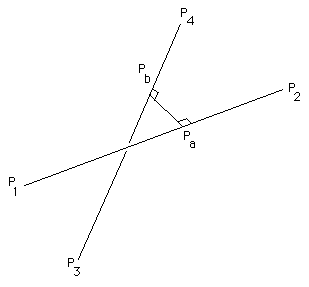
\includegraphics[height=5cm]{Pics/EdgeEdgeIntersection.png}
\end{frame}

\begin{slide}{Finding intersections}{Edge-to-edge intersections}{
\item The connecting axis is perpendicular to the both edges, so
$\left\{ \begin{matrix}
(P_a - P_b) \cdot D_1 &=& 0 \\
(P_a - P_b) \cdot D_2 &=& 0
\end{matrix} \right.$
\pause 
\item Expanding $P_a$ and $P_b$ results in
$\left\{ \begin{matrix}
(P_1 + \mu_a D_1 - P_2 - \mu_b D_2) \cdot D_1 &=& 0 \\
(P_1 + \mu_a D_1 - P_2 - \mu_b D_2) \cdot D_2 &=& 0
\end{matrix} \right.$
}\end{slide}

\begin{slide}{Finding intersections}{Edge-to-edge intersections}{
\item This is just a system with two unknowns and two equations; the dot products turn everything into numbers:
$\left\{ \begin{matrix}
(P_1 + \mu_a D_1 - P_2 - \mu_b D_2) \cdot D_1 &=& 0 \\
(P_1 + \mu_a D_1 - P_2 - \mu_b D_2) \cdot D_2 &=& 0
\end{matrix} \right.$
\item The full (tedious) derivation of the solutions is shown in \url{http://paulbourke.net/geometry/pointlineplane/}
}\end{slide}

\section{Assignment}
\begin{slide}{Assignment}{Assignment}{
\item Before the end of next week
\item Group-work archive/video on Natschool or uploaded somewhere else and linked in your report
\item Individual report by each of you on Natschool
\item Build a narrow phase collision detector that can compute the contact manifold
}\end{slide}

\begin{frame}{That's it}
\center
\fontsize{18pt}{7.2}\selectfont
Thank you!
\end{frame}

\end{document}


\begin{slide}{SECTION}{SLIDE}{
\item i
}\end{slide}

\begin{frame}[fragile]{SLIDE}
\begin{lstlisting}
CODE
\end{lstlisting}
\end{frame}

\begin{frame}{SLIDE}
\center
%\includegraphics[height=5cm]{Pics/recursive_multiplier.png}
\end{frame}
